
%% bare_jrnl.tex
%% V1.3
%% 2007/01/11
%% by Michael Shell
%% see http://www.michaelshell.org/
%% for current contact information.
%%
%% This is a skeleton file demonstrating the use of IEEEtran.cls
%% (requires IEEEtran.cls version 1.7 or later) with an IEEE journal paper.
%%
%% Support sites:
%% http://www.michaelshell.org/tex/ieeetran/
%% http://www.ctan.org/tex-archive/macros/latex/contrib/IEEEtran/
%% and
%% http://www.ieee.org/



% *** Authors should verify (and, if needed, correct) their LaTeX system  ***
% *** with the testflow diagnostic prior to trusting their LaTeX platform ***
% *** with production work. IEEE's font choices can trigger bugs that do  ***
% *** not appear when using other class files.                            ***
% The testflow support page is at:
% http://www.michaelshell.org/tex/testflow/


%%*************************************************************************
%% Legal Notice:
%% This code is offered as-is without any warranty either expressed or
%% implied; without even the implied warranty of MERCHANTABILITY or
%% FITNESS FOR A PARTICULAR PURPOSE! 
%% User assumes all risk.
%% In no event shall IEEE or any contributor to this code be liable for
%% any damages or losses, including, but not limited to, incidental,
%% consequential, or any other damages, resulting from the use or misuse
%% of any information contained here.
%%
%% All comments are the opinions of their respective authors and are not
%% necessarily endorsed by the IEEE.
%%
%% This work is distributed under the LaTeX Project Public License (LPPL)
%% ( http://www.latex-project.org/ ) version 1.3, and may be freely used,
%% distributed and modified. A copy of the LPPL, version 1.3, is included
%% in the base LaTeX documentation of all distributions of LaTeX released
%% 2003/12/01 or later.
%% Retain all contribution notices and credits.
%% ** Modified files should be clearly indicated as such, including  **
%% ** renaming them and changing author support contact information. **
%%
%% File list of work: IEEEtran.cls, IEEEtran_HOWTO.pdf, bare_adv.tex,
%%                    bare_conf.tex, bare_jrnl.tex, bare_jrnl_compsoc.tex
%%*************************************************************************

% Note that the a4paper option is mainly intended so that authors in
% countries using A4 can easily print to A4 and see how their papers will
% look in print - the typesetting of the document will not typically be
% affected with changes in paper size (but the bottom and side margins will).
% Use the testflow package mentioned above to verify correct handling of
% both paper sizes by the user's LaTeX system.
%
% Also note that the "draftcls" or "draftclsnofoot", not "draft", option
% should be used if it is desired that the figures are to be displayed in
% draft mode.
%
\documentclass[journal]{IEEEtran}
\usepackage{blindtext}
\usepackage{graphicx}
\usepackage{epstopdf}
\usepackage{cite}
\usepackage{amsmath}
\usepackage{array}
\usepackage[textsize=small]{todonotes}

% Some very useful LaTeX packages include:
% (uncomment the ones you want to load)


% *** MISC UTILITY PACKAGES ***
%
%\usepackage{ifpdf}
% Heiko Oberdiek's ifpdf.sty is very useful if you need conditional
% compilation based on whether the output is pdf or dvi.
% usage:
% \ifpdf
%   % pdf code
% \else
%   % dvi code
% \fi
% The latest version of ifpdf.sty can be obtained from:
% http://www.ctan.org/tex-archive/macros/latex/contrib/oberdiek/
% Also, note that IEEEtran.cls V1.7 and later provides a builtin
% \ifCLASSINFOpdf conditional that works the same way.
% When switching from latex to pdflatex and vice-versa, the compiler may
% have to be run twice to clear warning/error messages.






% *** CITATION PACKAGES ***
%
%\usepackage{cite}
% cite.sty was written by Donald Arseneau
% V1.6 and later of IEEEtran pre-defines the format of the cite.sty package
% \cite{} output to follow that of IEEE. Loading the cite package will
% result in citation numbers being automatically sorted and properly
% "compressed/ranged". e.g., [1], [9], [2], [7], [5], [6] without using
% cite.sty will become [1], [2], [5]--[7], [9] using cite.sty. cite.sty's
% \cite will automatically add leading space, if needed. Use cite.sty's
% noadjust option (cite.sty V3.8 and later) if you want to turn this off.
% cite.sty is already installed on most LaTeX systems. Be sure and use
% version 4.0 (2003-05-27) and later if using hyperref.sty. cite.sty does
% not currently provide for hyperlinked citations.
% The latest version can be obtained at:
% http://www.ctan.org/tex-archive/macros/latex/contrib/cite/
% The documentation is contained in the cite.sty file itself.






% *** GRAPHICS RELATED PACKAGES ***
%
\ifCLASSINFOpdf
  % \usepackage[pdftex]{graphicx}
  % declare the path(s) where your graphic files are
  % \graphicspath{{../pdf/}{../jpeg/}}
  % and their extensions so you won't have to specify these with
  % every instance of \includegraphics
  % \DeclareGraphicsExtensions{.pdf,.jpeg,.png}
\else
  % or other class option (dvipsone, dvipdf, if not using dvips). graphicx
  % will default to the driver specified in the system graphics.cfg if no
  % driver is specified.
  % \usepackage[dvips]{graphicx}
  % declare the path(s) where your graphic files are
  % \graphicspath{{../eps/}}
  % and their extensions so you won't have to specify these with
  % every instance of \includegraphics
  % \DeclareGraphicsExtensions{.eps}
\fi
% graphicx was written by David Carlisle and Sebastian Rahtz. It is
% required if you want graphics, photos, etc. graphicx.sty is already
% installed on most LaTeX systems. The latest version and documentation can
% be obtained at: 
% http://www.ctan.org/tex-archive/macros/latex/required/graphics/
% Another good source of documentation is "Using Imported Graphics in
% LaTeX2e" by Keith Reckdahl which can be found as epslatex.ps or
% epslatex.pdf at: http://www.ctan.org/tex-archive/info/
%
% latex, and pdflatex in dvi mode, support graphics in encapsulated
% postscript (.eps) format. pdflatex in pdf mode supports graphics
% in .pdf, .jpeg, .png and .mps (metapost) formats. Users should ensure
% that all non-photo figures use a vector format (.eps, .pdf, .mps) and
% not a bitmapped formats (.jpeg, .png). IEEE frowns on bitmapped formats
% which can result in "jaggedy"/blurry rendering of lines and letters as
% well as large increases in file sizes.
%
% You can find documentation about the pdfTeX application at:
% http://www.tug.org/applications/pdftex





% *** MATH PACKAGES ***
%
%\usepackage[cmex10]{amsmath}
% A popular package from the American Mathematical Society that provides
% many useful and powerful commands for dealing with mathematics. If using
% it, be sure to load this package with the cmex10 option to ensure that
% only type 1 fonts will utilized at all point sizes. Without this option,
% it is possible that some math symbols, particularly those within
% footnotes, will be rendered in bitmap form which will result in a
% document that can not be IEEE Xplore compliant!
%
% Also, note that the amsmath package sets \interdisplaylinepenalty to 10000
% thus preventing page breaks from occurring within multiline equations. Use:
\interdisplaylinepenalty=2500
% after loading amsmath to restore such page breaks as IEEEtran.cls normally
% does. amsmath.sty is already installed on most LaTeX systems. The latest
% version and documentation can be obtained at:
% http://www.ctan.org/tex-archive/macros/latex/required/amslatex/math/





% *** SPECIALIZED LIST PACKAGES ***
%
%\usepackage{algorithmic}
% algorithmic.sty was written by Peter Williams and Rogerio Brito.
% This package provides an algorithmic environment fo describing algorithms.
% You can use the algorithmic environment in-text or within a figure
% environment to provide for a floating algorithm. Do NOT use the algorithm
% floating environment provided by algorithm.sty (by the same authors) or
% algorithm2e.sty (by Christophe Fiorio) as IEEE does not use dedicated
% algorithm float types and packages that provide these will not provide
% correct IEEE style captions. The latest version and documentation of
% algorithmic.sty can be obtained at:
% http://www.ctan.org/tex-archive/macros/latex/contrib/algorithms/
% There is also a support site at:
% http://algorithms.berlios.de/index.html
% Also of interest may be the (relatively newer and more customizable)
% algorithmicx.sty package by Szasz Janos:
% http://www.ctan.org/tex-archive/macros/latex/contrib/algorithmicx/




% *** ALIGNMENT PACKAGES ***
%
%\usepackage{array}
% Frank Mittelbach's and David Carlisle's array.sty patches and improves
% the standard LaTeX2e array and tabular environments to provide better
% appearance and additional user controls. As the default LaTeX2e table
% generation code is lacking to the point of almost being broken with
% respect to the quality of the end results, all users are strongly
% advised to use an enhanced (at the very least that provided by array.sty)
% set of table tools. array.sty is already installed on most systems. The
% latest version and documentation can be obtained at:
% http://www.ctan.org/tex-archive/macros/latex/required/tools/


\usepackage{mdwmath}
\usepackage{mdwtab}
% Also highly recommended is Mark Wooding's extremely powerful MDW tools,
% especially mdwmath.sty and mdwtab.sty which are used to format equations
% and tables, respectively. The MDWtools set is already installed on most
% LaTeX systems. The lastest version and documentation is available at:
% http://www.ctan.org/tex-archive/macros/latex/contrib/mdwtools/


% IEEEtran contains the IEEEeqnarray family of commands that can be used to
% generate multiline equations as well as matrices, tables, etc., of high
% quality.


\usepackage{eqparbox}
% Also of notable interest is Scott Pakin's eqparbox package for creating
% (automatically sized) equal width boxes - aka "natural width parboxes".
% Available at:
% http://www.ctan.org/tex-archive/macros/latex/contrib/eqparbox/





% *** SUBFIGURE PACKAGES ***
%\usepackage[tight,footnotesize]{subfigure}
% subfigure.sty was written by Steven Douglas Cochran. This package makes it
% easy to put subfigures in your figures. e.g., "Figure 1a and 1b". For IEEE
% work, it is a good idea to load it with the tight package option to reduce
% the amount of white space around the subfigures. subfigure.sty is already
% installed on most LaTeX systems. The latest version and documentation can
% be obtained at:
% http://www.ctan.org/tex-archive/obsolete/macros/latex/contrib/subfigure/
% subfigure.sty has been superceeded by subfig.sty.



%\usepackage[caption=false]{caption}
%\usepackage[font=footnotesize]{subfig}
% subfig.sty, also written by Steven Douglas Cochran, is the modern
% replacement for subfigure.sty. However, subfig.sty requires and
% automatically loads Axel Sommerfeldt's caption.sty which will override
% IEEEtran.cls handling of captions and this will result in nonIEEE style
% figure/table captions. To prevent this problem, be sure and preload
% caption.sty with its "caption=false" package option. This is will preserve
% IEEEtran.cls handing of captions. Version 1.3 (2005/06/28) and later 
% (recommended due to many improvements over 1.2) of subfig.sty supports
% the caption=false option directly:
\usepackage[caption=false,font=footnotesize]{subfig}
%
% The latest version and documentation can be obtained at:
% http://www.ctan.org/tex-archive/macros/latex/contrib/subfig/
% The latest version and documentation of caption.sty can be obtained at:
% http://www.ctan.org/tex-archive/macros/latex/contrib/caption/




% *** FLOAT PACKAGES ***
%
\usepackage{fixltx2e}
% fixltx2e, the successor to the earlier fix2col.sty, was written by
% Frank Mittelbach and David Carlisle. This package corrects a few problems
% in the LaTeX2e kernel, the most notable of which is that in current
% LaTeX2e releases, the ordering of single and double column floats is not
% guaranteed to be preserved. Thus, an unpatched LaTeX2e can allow a
% single column figure to be placed prior to an earlier double column
% figure. The latest version and documentation can be found at:
% http://www.ctan.org/tex-archive/macros/latex/base/



\usepackage{stfloats}
% stfloats.sty was written by Sigitas Tolusis. This package gives LaTeX2e
% the ability to do double column floats at the bottom of the page as well
% as the top. (e.g., "\begin{figure*}[!b]" is not normally possible in
% LaTeX2e). It also provides a command:
%\fnbelowfloat
% to enable the placement of footnotes below bottom floats (the standard
% LaTeX2e kernel puts them above bottom floats). This is an invasive package
% which rewrites many portions of the LaTeX2e float routines. It may not work
% with other packages that modify the LaTeX2e float routines. The latest
% version and documentation can be obtained at:
% http://www.ctan.org/tex-archive/macros/latex/contrib/sttools/
% Documentation is contained in the stfloats.sty comments as well as in the
% presfull.pdf file. Do not use the stfloats baselinefloat ability as IEEE
% does not allow \baselineskip to stretch. Authors submitting work to the
% IEEE should note that IEEE rarely uses double column equations and
% that authors should try to avoid such use. Do not be tempted to use the
% cuted.sty or midfloat.sty packages (also by Sigitas Tolusis) as IEEE does
% not format its papers in such ways.


%\ifCLASSOPTIONcaptionsoff
%  \usepackage[nomarkers]{endfloat}
% \let\MYoriglatexcaption\caption
% \renewcommand{\caption}[2][\relax]{\MYoriglatexcaption[#2]{#2}}
%\fi
% endfloat.sty was written by James Darrell McCauley and Jeff Goldberg.
% This package may be useful when used in conjunction with IEEEtran.cls'
% captionsoff option. Some IEEE journals/societies require that submissions
% have lists of figures/tables at the end of the paper and that
% figures/tables without any captions are placed on a page by themselves at
% the end of the document. If needed, the draftcls IEEEtran class option or
% \CLASSINPUTbaselinestretch interface can be used to increase the line
% spacing as well. Be sure and use the nomarkers option of endfloat to
% prevent endfloat from "marking" where the figures would have been placed
% in the text. The two hack lines of code above are a slight modification of
% that suggested by in the endfloat docs (section 8.3.1) to ensure that
% the full captions always appear in the list of figures/tables - even if
% the user used the short optional argument of \caption[]{}.
% IEEE papers do not typically make use of \caption[]'s optional argument,
% so this should not be an issue. A similar trick can be used to disable
% captions of packages such as subfig.sty that lack options to turn off
% the subcaptions:
% For subfig.sty:
% \let\MYorigsubfloat\subfloat
% \renewcommand{\subfloat}[2][\relax]{\MYorigsubfloat[]{#2}}
% For subfigure.sty:
% \let\MYorigsubfigure\subfigure
% \renewcommand{\subfigure}[2][\relax]{\MYorigsubfigure[]{#2}}
% However, the above trick will not work if both optional arguments of
% the \subfloat/subfig command are used. Furthermore, there needs to be a
% description of each subfigure *somewhere* and endfloat does not add
% subfigure captions to its list of figures. Thus, the best approach is to
% avoid the use of subfigure captions (many IEEE journals avoid them anyway)
% and instead reference/explain all the subfigures within the main caption.
% The latest version of endfloat.sty and its documentation can obtained at:
% http://www.ctan.org/tex-archive/macros/latex/contrib/endfloat/
%
% The IEEEtran \ifCLASSOPTIONcaptionsoff conditional can also be used
% later in the document, say, to conditionally put the References on a 
% page by themselves.





% *** PDF, URL AND HYPERLINK PACKAGES ***
%
%\usepackage{url}
% url.sty was written by Donald Arseneau. It provides better support for
% handling and breaking URLs. url.sty is already installed on most LaTeX
% systems. The latest version can be obtained at:
% http://www.ctan.org/tex-archive/macros/latex/contrib/misc/
% Read the url.sty source comments for usage information. Basically,
% \url{my_url_here}.





% *** Do not adjust lengths that control margins, column widths, etc. ***
% *** Do not use packages that alter fonts (such as pslatex).         ***
% There should be no need to do such things with IEEEtran.cls V1.6 and later.
% (Unless specifically asked to do so by the journal or conference you plan
% to submit to, of course. )


% correct bad hyphenation here
\hyphenation{op-tical net-works semi-conduc-tor}


\begin{document}
%
% paper title
% can use linebreaks \\ within to get better formatting as desired
\title{IEEE Journal Template Example}
%
%
% author names and IEEE memberships
% note positions of commas and nonbreaking spaces ( ~ ) LaTeX will not break
% a structure at a ~ so this keeps an author's name from being broken across
% two lines.
% use \thanks{} to gain access to the first footnote area
% a separate \thanks must be used for each paragraph as LaTeX2e's \thanks
% was not built to handle multiple paragraphs
%

\author{Michael~Shell,~\IEEEmembership{Member,~IEEE,}
        John~Doe,~\IEEEmembership{Fellow,~OSA,}
        and~Jane~Doe,~\IEEEmembership{Life~Fellow,~IEEE}% <-this % stops a space
\thanks{M. Shell is with the Department
of Electrical and Computer Engineering, Georgia Institute of Technology, Atlanta,
GA, 30332 USA e-mail: (see http://www.michaelshell.org/contact.html).}% <-this % stops a space
\thanks{J. Doe and J. Doe are with Anonymous University.}% <-this % stops a space
\thanks{Manuscript received April 19, 2005; revised January 11, 2007.}}

% note the % following the last \IEEEmembership and also \thanks - 
% these prevent an unwanted space from occurring between the last author name
% and the end of the author line. i.e., if you had this:
% 
% \author{....lastname \thanks{...} \thanks{...} }
%                     ^------------^------------^----Do not want these spaces!
%
% a space would be appended to the last name and could cause every name on that
% line to be shifted left slightly. This is one of those "LaTeX things". For
% instance, "\textbf{A} \textbf{B}" will typeset as "A B" not "AB". To get
% "AB" then you have to do: "\textbf{A}\textbf{B}"
% \thanks is no different in this regard, so shield the last } of each \thanks
% that ends a line with a % and do not let a space in before the next \thanks.
% Spaces after \IEEEmembership other than the last one are OK (and needed) as
% you are supposed to have spaces between the names. For what it is worth,
% this is a minor point as most people would not even notice if the said evil
% space somehow managed to creep in.



% The paper headers
\markboth{Journal of \LaTeX\ Class Files,~Vol.~6, No.~1, January~2007}%
{Shell \MakeLowercase{\textit{et al.}}: Bare Demo of IEEEtran.cls for Journals}
% The only time the second header will appear is for the odd numbered pages
% after the title page when using the twoside option.
% 
% *** Note that you probably will NOT want to include the author's ***
% *** name in the headers of peer review papers.                   ***
% You can use \ifCLASSOPTIONpeerreview for conditional compilation here if
% you desire.




% If you want to put a publisher's ID mark on the page you can do it like
% this:
%\IEEEpubid{0000--0000/00\$00.00~\copyright~2007 IEEE}
% Remember, if you use this you must call \IEEEpubidadjcol in the second
% column for its text to clear the IEEEpubid mark.



% use for special paper notices
%\IEEEspecialpapernotice{(Invited Paper)}




% make the title area
\maketitle


\begin{abstract}
%\boldmath
\blindtext[1]
\end{abstract}
% IEEEtran.cls defaults to using nonbold math in the Abstract.
% This preserves the distinction between vectors and scalars. However,
% if the journal you are submitting to favors bold math in the abstract,
% then you can use LaTeX's standard command \boldmath at the very start
% of the abstract to achieve this. Many IEEE journals frown on math
% in the abstract anyway.

% Note that keywords are not normally used for peerreview papers.
\begin{IEEEkeywords}
IEEEtran, journal, \LaTeX, paper, template.
\end{IEEEkeywords}






% For peer review papers, you can put extra information on the cover
% page as needed:
% \ifCLASSOPTIONpeerreview
% \begin{center} \bfseries EDICS Category: 3-BBND \end{center}
% \fi
%
% For peerreview papers, this IEEEtran command inserts a page break and
% creates the second title. It will be ignored for other modes.
\IEEEpeerreviewmaketitle



\section{Introduction}

The increase of the aircraft operational costs associated with the fuel consumption drives the development of new aircraft technologies \citep{Babikian2002}. In this scenario, the aviation market has changed the design perception regarding the electrical system, replacing hydraulic and pneumatic’s power source to equivalent electrical ones, creating the concept of the More Electrical Aircraft (MEA) \citep{Moir1999}.

This context raised the relevance of the EPGDS (Electrical Power Generation and Distribution System) in the role of aircraft operational safety. Thus, the electrical system needs to have a greater reliability and operates in such a way to avoid failures of the equipment connected to the grid. However, the increase of the amount of non-linear loads has raised the harmonic distortion content introduced in the EPGDS \citep{Singer2012}, diminishing the power quality and becoming a subject of study in aircraft operational safety. 

To improve the power quality with the reduction of the total harmonic distortion (THD), some conditioners must be connected in the equipment power input and/or in the distribution grid. The implementation of these conditioners must consider the reliability, weight and cost to be feasible in aircraft design.

In this context, some topologies to increase the power quality are already used in the aircraft electrical system, such as the multi-pulse rectifiers \citep{Zhu2014,Gong2003,Lobo2005}. However, its weight and volume make this topology applicable only to specific equipment.

With the increase of the non-linear loads applied to the electrical grid, along with the requirements to ensure power quality, some alternatives of power factor correction have been proposed. In this scenario, the use of a shunt active filter applied in an aircraft is an item of recent study, considering different active filters topologies \citep{Chen2012research,Chen2012novel,Chen2012control}.

This article analyses the use of a shunt active filter to improve the power quality in the aircraft EPGDS. It starts by reviewing the active filter operation, the instantaneous power theory, and continues discussing control techniques. A simulation is presented to analyze the shunt active filter operation with three electrohydraulic actuators (EHA), which are non-linear loads used to control the aircraft latero-directional and longitudinal aerodynamics surfaces. The simulation model is compounded by the electrical generation and distribution system connected to EHAs with their respective shunt active filters.


\section{Power Quality in Aircraft}\label{sec:Power_Quality}

The power quality in aircraft EPGDS is a concern which regards the airworthiness. The electrical equipment used in aircraft design must be qualified to ensure the proper operation and integration. Thereby, the power quality is one of the subjects considered in the qualification tests, which are specified by standard test procedures issued by aeronautical authorities. The most used qualifications standards for electrical systems are the MIL-STD 704, which qualifies the EPGDS, and the DO-160 - Section 16, which qualifies the embedded electrical equipment. To ensure the proper equipment integration, the EPGDS  and equipment must comply with these standards.

The non-linear loads inject harmonic distortion content in the system, inducing degradation in the power quality and decreasing the power factor. Furthermore, the increase in the number of electrical equipment connected in the grid enhances the degradation of the power quality. Thus, techniques for power factor correction must be applied in the EPGDS to limit the system operation within the constraints of aeronautical standards.

Some techniques are already used in aircraft electrical system to increase the power factor and power quality. One of these techniques is the use of multi-pulse converters, which is most employed in high capacity loads rectifiers to improve the power quality. However, despite of the good reliability, they are bulky and heavy. There are some other topologies that are useful for harmonic content reduction, but their characteristics do not make them feasible to operate in the aircraft systems. Some of these topologies are the passive filters and power factor correction (PFC) converters. For the passive filters, despite of good reliability and low cost, the high weight is the main problem to its implementation in aircraft \citep{Barruel2004}. For the PFC converters, the downside lies in the low reliability and low density of energy conditioned \citep{Zhu2014,Gong2003,Lobo2005}. 

In this scenario, the active filter, due to its features as lightweight and fast response to load variation, appears to be a feasible topology to reduce the harmonic content and increase the power factor \citep{Zhu2014,Chen2012control,Karatzaferis2013}. There are some drawbacks in its use, as the high complexity and low reliability, but the advances in power electronics are making them practical to be implemented in aircraft electrical system \citep{Abdelhafez2009}.







\section{Active Filters}

The active filter operates creating waveforms to interact with the voltages and currents presented in the electrical grid to establish a power factor equal to one. This is accomplished by measuring the voltage waveforms from the power source and the current waveforms from the load, and then using these parameters on the instantaneous power theory to determine the current reference as an input to be set in a compensator. The compensator injects current waveforms in the circuit with symmetrical values of the components which degrades the power factor. The typical system compounded by a non-linear load with an active filter is presented in Fig. \ref{fig:compensador.png}.

\begin{figure}[!h]
\centering
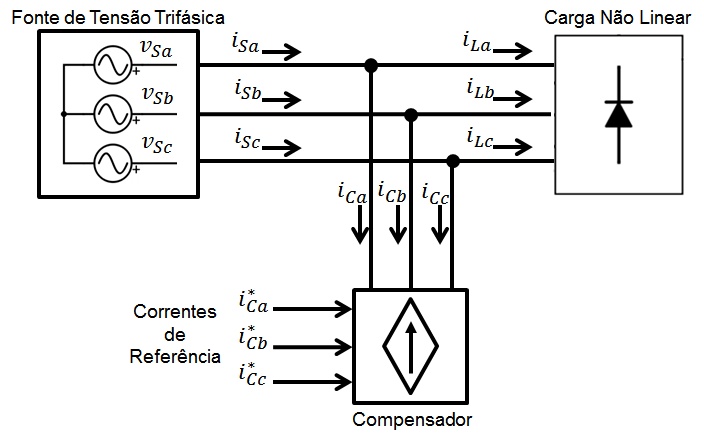
\includegraphics[width=2.8in]{Figures/compensador.png}
\caption{Simulation Results}
\label{fig:compensador.png}
\end{figure}

%\begin{figure}
%	\centering
%	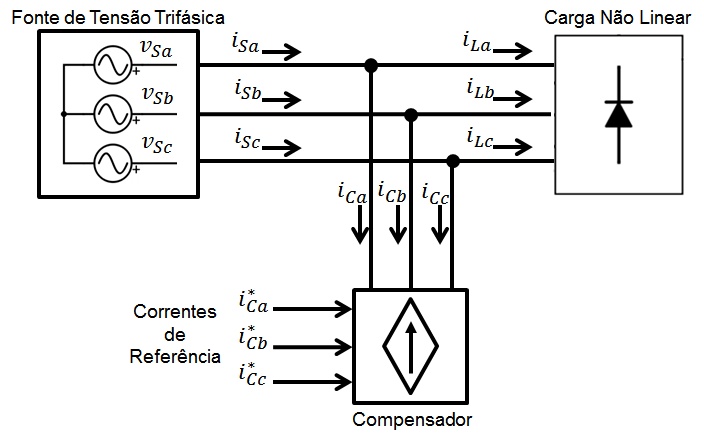
\includegraphics[width=0.4\textwidth]{Figures/compensador.png}
%	\caption{Simulation Results}
%	\label{fig:compensador.png}
%\end{figure}


\subsection{Instantaneous Power Theory}

The instantaneous power theory was presented by Akagi \cite{Akagi}, which proposed some new concepts for the instantaneous active and reactive power. This theory can be used in three phase, three or four wire system and in steady or transient state \cite{Akagi,Akagi}. In this theory, the manipulation of the active and reactive power calculations brings a tool to determine the currents that carry some content which degrade the power factor, such as harmonic distortion and phase shift.
Considering a three-phase system, composed by the phases $a$, $b$ and $c$, the instantaneous power theory is based in the coordinates transformation from the $abc$ to $\alpha \beta 0 $. This is known as the Clarke Transformation and is shown in eq. (2) \ref{eq:Clarke}.

\begin{equation}
\begin{aligned}
\begin{bmatrix}
v_0\\
v_\alpha\\
v_\beta
\end{bmatrix}
& = \sqrt{\dfrac{2}{3}}
\begin{bmatrix}
\dfrac{1}{\sqrt{2}}	& \dfrac{1}{\sqrt{2}}	& \dfrac{1}{\sqrt{2}}		\\[2ex]
1					& -\dfrac{1}{2}			& -\dfrac{1}{2}				\\[2ex]
0					& \dfrac{\sqrt{3}}{2}	& -\dfrac{\sqrt{3}}{2}
\end{bmatrix}
\begin{bmatrix}
v_a\\
v_b\\
v_c
\end{bmatrix}
;\\
\begin{bmatrix}
i_0\\
i_\alpha\\
i_\beta
\end{bmatrix}
& = \sqrt{\dfrac{2}{3}}
\begin{bmatrix}
\dfrac{1}{\sqrt{2}}	& \dfrac{1}{\sqrt{2}}	& \dfrac{1}{\sqrt{2}}		\\[2ex]
1					& -\dfrac{1}{2}			& -\dfrac{1}{2}				\\[2ex]
0					& \dfrac{\sqrt{3}}{2}	& -\dfrac{\sqrt{3}}{2}
\end{bmatrix}
\begin{bmatrix}
i_a\\
i_b\\
i_c
\end{bmatrix}
\label{eq:Clarke}
\end{aligned}
\end{equation} 

According to \cite{Akagi}, the instantaneous power is defined as shown in eq (3) \ref{eq:pq_0}, where the $p_0$, $p$ and $q$ are the instantaneous zero-sequence power, the active instantaneous power and the reactive instantaneous power, respectively \cite{Akagi,Peng1996}.

\begin{equation}
\begin{bmatrix}
p_0\\
p\\
q
\end{bmatrix}=
\begin{bmatrix}
v_0		&	0			&	0\\
0		&	v_{\alpha}	&	v_{\beta}\\
0		&	v_{\beta}	&	-v_{\alpha}
\end{bmatrix}
\begin{bmatrix}
i_{0}\\
i_{\alpha}\\
i_{\beta}
\end{bmatrix}
\label{eq:pq_0}
\end{equation} 

Considering a system without zero-sequence voltage and/or current, such as the aircraft electrical system, the eq (3) can be simplified as the eq (4), where the instantaneous zero-sequence power is absent.

\begin{equation}
\begin{bmatrix}
p\\
q
\end{bmatrix}=
\begin{bmatrix}
v_{\alpha}	&	v_{\beta}\\
v_{\beta}	&	-v_{\alpha}
\end{bmatrix}
\begin{bmatrix}
i_{\alpha}\\
i_{\beta}
\end{bmatrix}
\label{eq:pq}
\end{equation} 

The reverse calculation, i.e., the determination of the currents $i_{\alpha}$ and $i_{\beta}$ when the voltages $v_{alpha}$ and $v_{\beta}$ and the instantaneous power $p$ and $q$ are known is presented in eq. (5) \ref{eq:i_alphabeta}.

\begin{equation}
\begin{bmatrix}
i_{\alpha}\\
i_{\beta}
\end{bmatrix}=
\dfrac{1}{v_{\alpha}^2+v_{\beta}^2}
\begin{bmatrix}
v_{\alpha}	&	v_{\beta}\\
v_{\beta}	&	-v_{\alpha}
\end{bmatrix}
\begin{bmatrix}
p\\
q
\end{bmatrix}
\label{eq:i_alphabeta}
\end{equation}

By definition, the active instantaneous power is composed by the energy that is swapped between two subsystems, whereas the reactive power is composed by the energy being swapped between the 3 phases of the system \cite{Akagi}. Furthermore, both $p$ and $q$ can be defined as a composition of an average ($\overline{p}$ and $\overline{q}$) and an oscillating ($\tilde{p}$ and $\tilde{q}$) values, as defined in eq. (6) \ref{eq:pq_m_o}.

\begin{equation}
\begin{aligned}
p = \overline{p} + \tilde{p}\\
q = \overline{q} + \tilde{q} 
\end{aligned}
\label{eq:pq_m_o}
\end{equation} 

To create an active filter to coordinate a power factor equal to 1, the only permitted power flowing in the transmission lines is the average value of the instantaneous active power ($\overline{p}$). To ensure this condition, the filter must inject in the lines currents which contains the symmetrical values of the instantaneous reactive power ($q$) and the oscillating portion of the instantaneous active power ($\tilde{p}$) created by the non-linear load. By doing this, these powers are cancelled in the same way as the current harmonic content. Thereby, the selection of power to be compensate and processed by the filter must contains the values of the $-\tilde{p}$ and $-q$ only.

The filter full operation is defined by the instantaneous power $p$ and $q$ calculation, followed by the selection of the power to be compensated, i.e., $-\tilde{p}$ and $-q$. Afterwards, the currents $i_{\alpha}$ and $i_{\beta}$ are calculated using the eq (5) \ref{eq:i_alphabeta} with the values $-\tilde{p}$ and $-q$, followed by the inverse Clarke transformation to acquire the current in $abc$ coordinates to be applied as a reference in the compensator. The whole active filter reference definition is shown in Fig. \ref{fig:diagrama_filtro.png}.

\begin{figure}[!th]
	\centering
	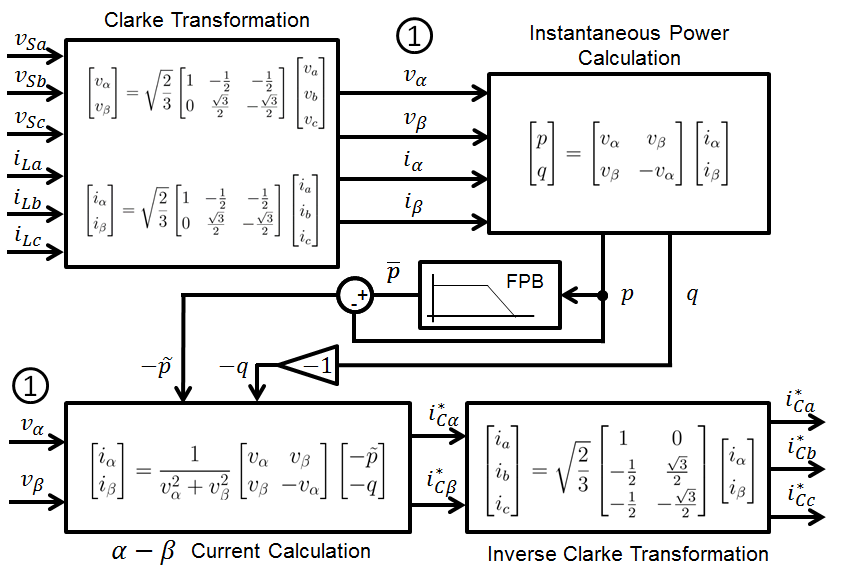
\includegraphics[width=3in]{Figures/diagrama_filtro.png}
	\caption{Simulation Results}
	\label{fig:diagrama_filtro.png}
\end{figure}

%\begin{figure}
%	\centering
%	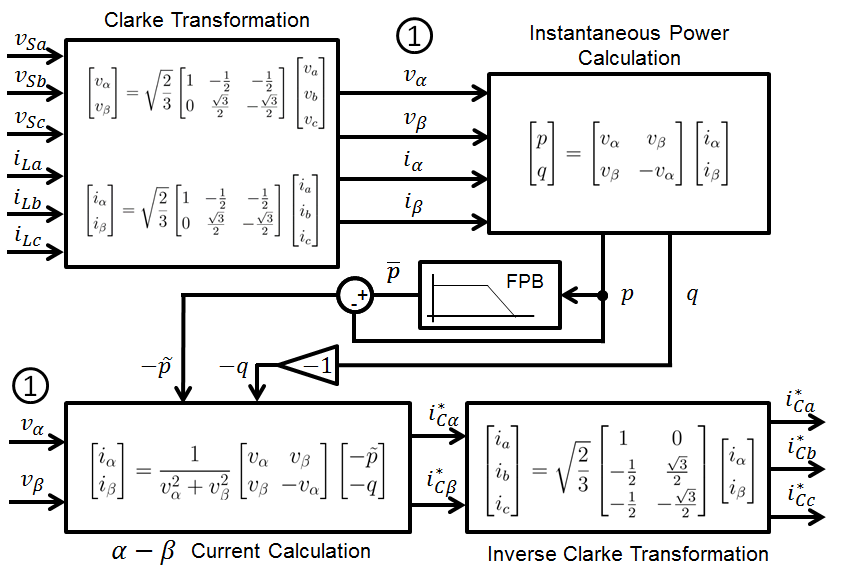
\includegraphics[width=0.47\textwidth]{Figures/diagrama_filtro.png}
%	\caption{Active filter reference definition}
%	\label{fig:diagrama_filtro.png}
%\end{figure}

\subsection{Control Strategy}

The active filter specified in Fig (7) \ref{fig:diagrama_filtro.png} presents very effective to set the current reference to be applied in the compensator for mitigation of the electrical system harmonic content. However, this calculation is valid to produce sinusoidal current waveforms only when the voltages measured and used in the filter input is pure sine waves. This happens since the filter operates in such way that only the mean value of the active instantaneous power flows in the circuit. Therefore, the use of a non-sinusoidal voltage waveform in the input of the filter requires a non-sinusoidal current waveform to establish the power flow with only $\overline{p}$.

In aircraft electrical power system, the voltage waveforms stated in the point of common connection (PCC) are presented as non-sinusoidal, however, they are still limited by the aeronautical standards. As the voltages used in the active filter are measured at the PCC or beyond this point, its operation is not optimal for power quality purposes, and, in some cases, it may decrease the power quality and operates unstably depending the levels of harmonic distortion presented in the voltages waveforms.

According to \cite{Akagi2007}, the p-q theory proves insufficient to satisfy the condition to create a current sine wave and an active instantaneous power flow consisted of only the its mean value, at the same time the voltage waveforms measured and presented on the PCC are previously distorted. To overcome this situation, a control strategy based on the use of a positive-sequence voltage detector is employed to ensure a sinusoidal current control. With this, the power flow between the load and the source is not defined as the mean value of the active instantaneous power, however, the control strategy relays on the appropriate sine wave current insertion in order to establish the proper power quality at the system.

This control is designed by the use of the positive-sequence voltage detector, which operates to extract the fundamental positive-sequence component from the distorted voltages. This component is required by the active filter to define the current shape to be applied in the electrical grid to create a sinusoidal waveform.

The positive-sequence voltage detector operates based on the p-q dual theory where it is used a phase locked loop (PLL) and the p-q theory to extract the fundamental frequency and amplitude of the distorted voltages. The PLL is show in Fig. \ref{fig:PLL.png} and operates defining the fundamental frequency and phase. The scheme shown in Fig. \ref{fig:detector_seq_positiva.png} uses the p-q theory and the information coming from the PLL to define the amplitude of the fundamental component to be used in the active filter calculations.

\begin{figure}[!th]
	\centering
	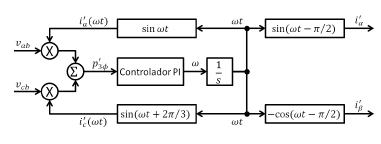
\includegraphics[width=3in]{Figures/PLL.png}
	\caption{Phase locked loop}
	\label{fig:PLL.png}
\end{figure}

\begin{figure}[!th]
	\centering
	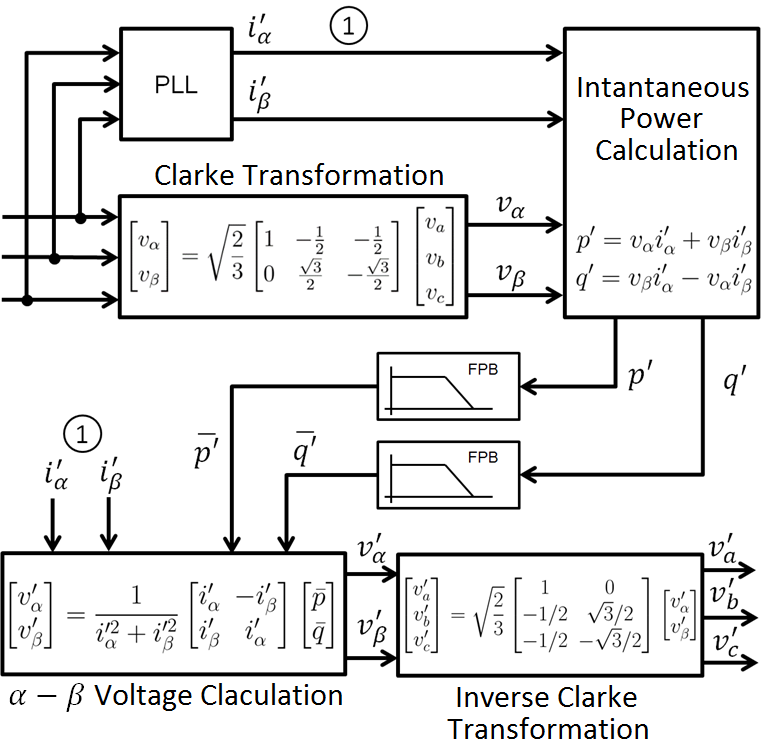
\includegraphics[width=3in]{Figures/detector_seq_positiva.png}
	\caption{Positive-sequence detector}
	\label{fig:detector_seq_positiva.png}
\end{figure}

In the operation of the active filter, some loss is presented in the circuit, mainly due to the VSC switching devices, which cause the voltage of the capacitor, locate in the converter DC side, to decrease. To avoid this voltage drop, a closed-loop design with a PI controller is applied in the active filter to define the power to compensate the system power loss. This closed-loop error signal is processed by the compensator, causing this to manage the power flow in the VSC to hold the capacitor voltage to specifically reference.


\section{Simulation of the Shunt Active Filter Operating with an Electrohidraulic Actuator}

The operation of the shunt active filter in an aircraft electrical system was evaluated by simulation. The system is composed by the generation and distribution system and some loads constituted by electrohydraulic actuators (EHAs) with shunt active filters connected to its respective inputs.

\subsection{Active Filter Model}

The shunt active filter consists of a Current Reference Calculator and a Compensator, as shown in Fig. \ref{fig:filtro_blocos_1.png}. This figure shows these parts with its respective internal sub-blocks. The Current Reference Calculator block is comprised by the Positive Sequence Detector (Fig. 4 \ref{fig:detector_seq_positiva.png}) and the Active Filter Reference Definition (Fig. 2 \ref{fig:diagrama_filtro.png}). These sub-blocks are responsible for the calculation algorithm (each sub-block presents its respective signals inputs and outputs) to determine the reference to be applied in the compensator. The Compensator is presented by the VSC with its respective hysteresis controller and capacitor voltage PI controller. This figure shows also the voltages and currents measurement probes connection in the electrical grid, where acquire the inputs for the active filter operaion.

The reference calculator block defines the proper reference to be applied in the compensator. Its inputs are the load currents and the grid voltages measurements, while its output is the reference applied to the compensator. The compensator block consists of a VSC with its capacitor DC voltage regulated by a closed-loop controller. The compensator also has the hysteresis controller, which creates the commands applied to the VSC switching devices.

The shunt active filter operation requires a passive capacitor filter applied in the transmission lines to eliminate the high frequency content injected in the system by the switching commutation \cite{Akagi2007}. Due to high switching commutation frequency, the passive filter is lightweight and does not impact significantly in the aircraft system. However, the presence of capacitors in the transmission lines may decrease the power factor due to current phase shift. To eliminate this, inductors may be applied in the lines to compensate the reactive power flow.

\begin{figure*}[!tb] %
	\centering
	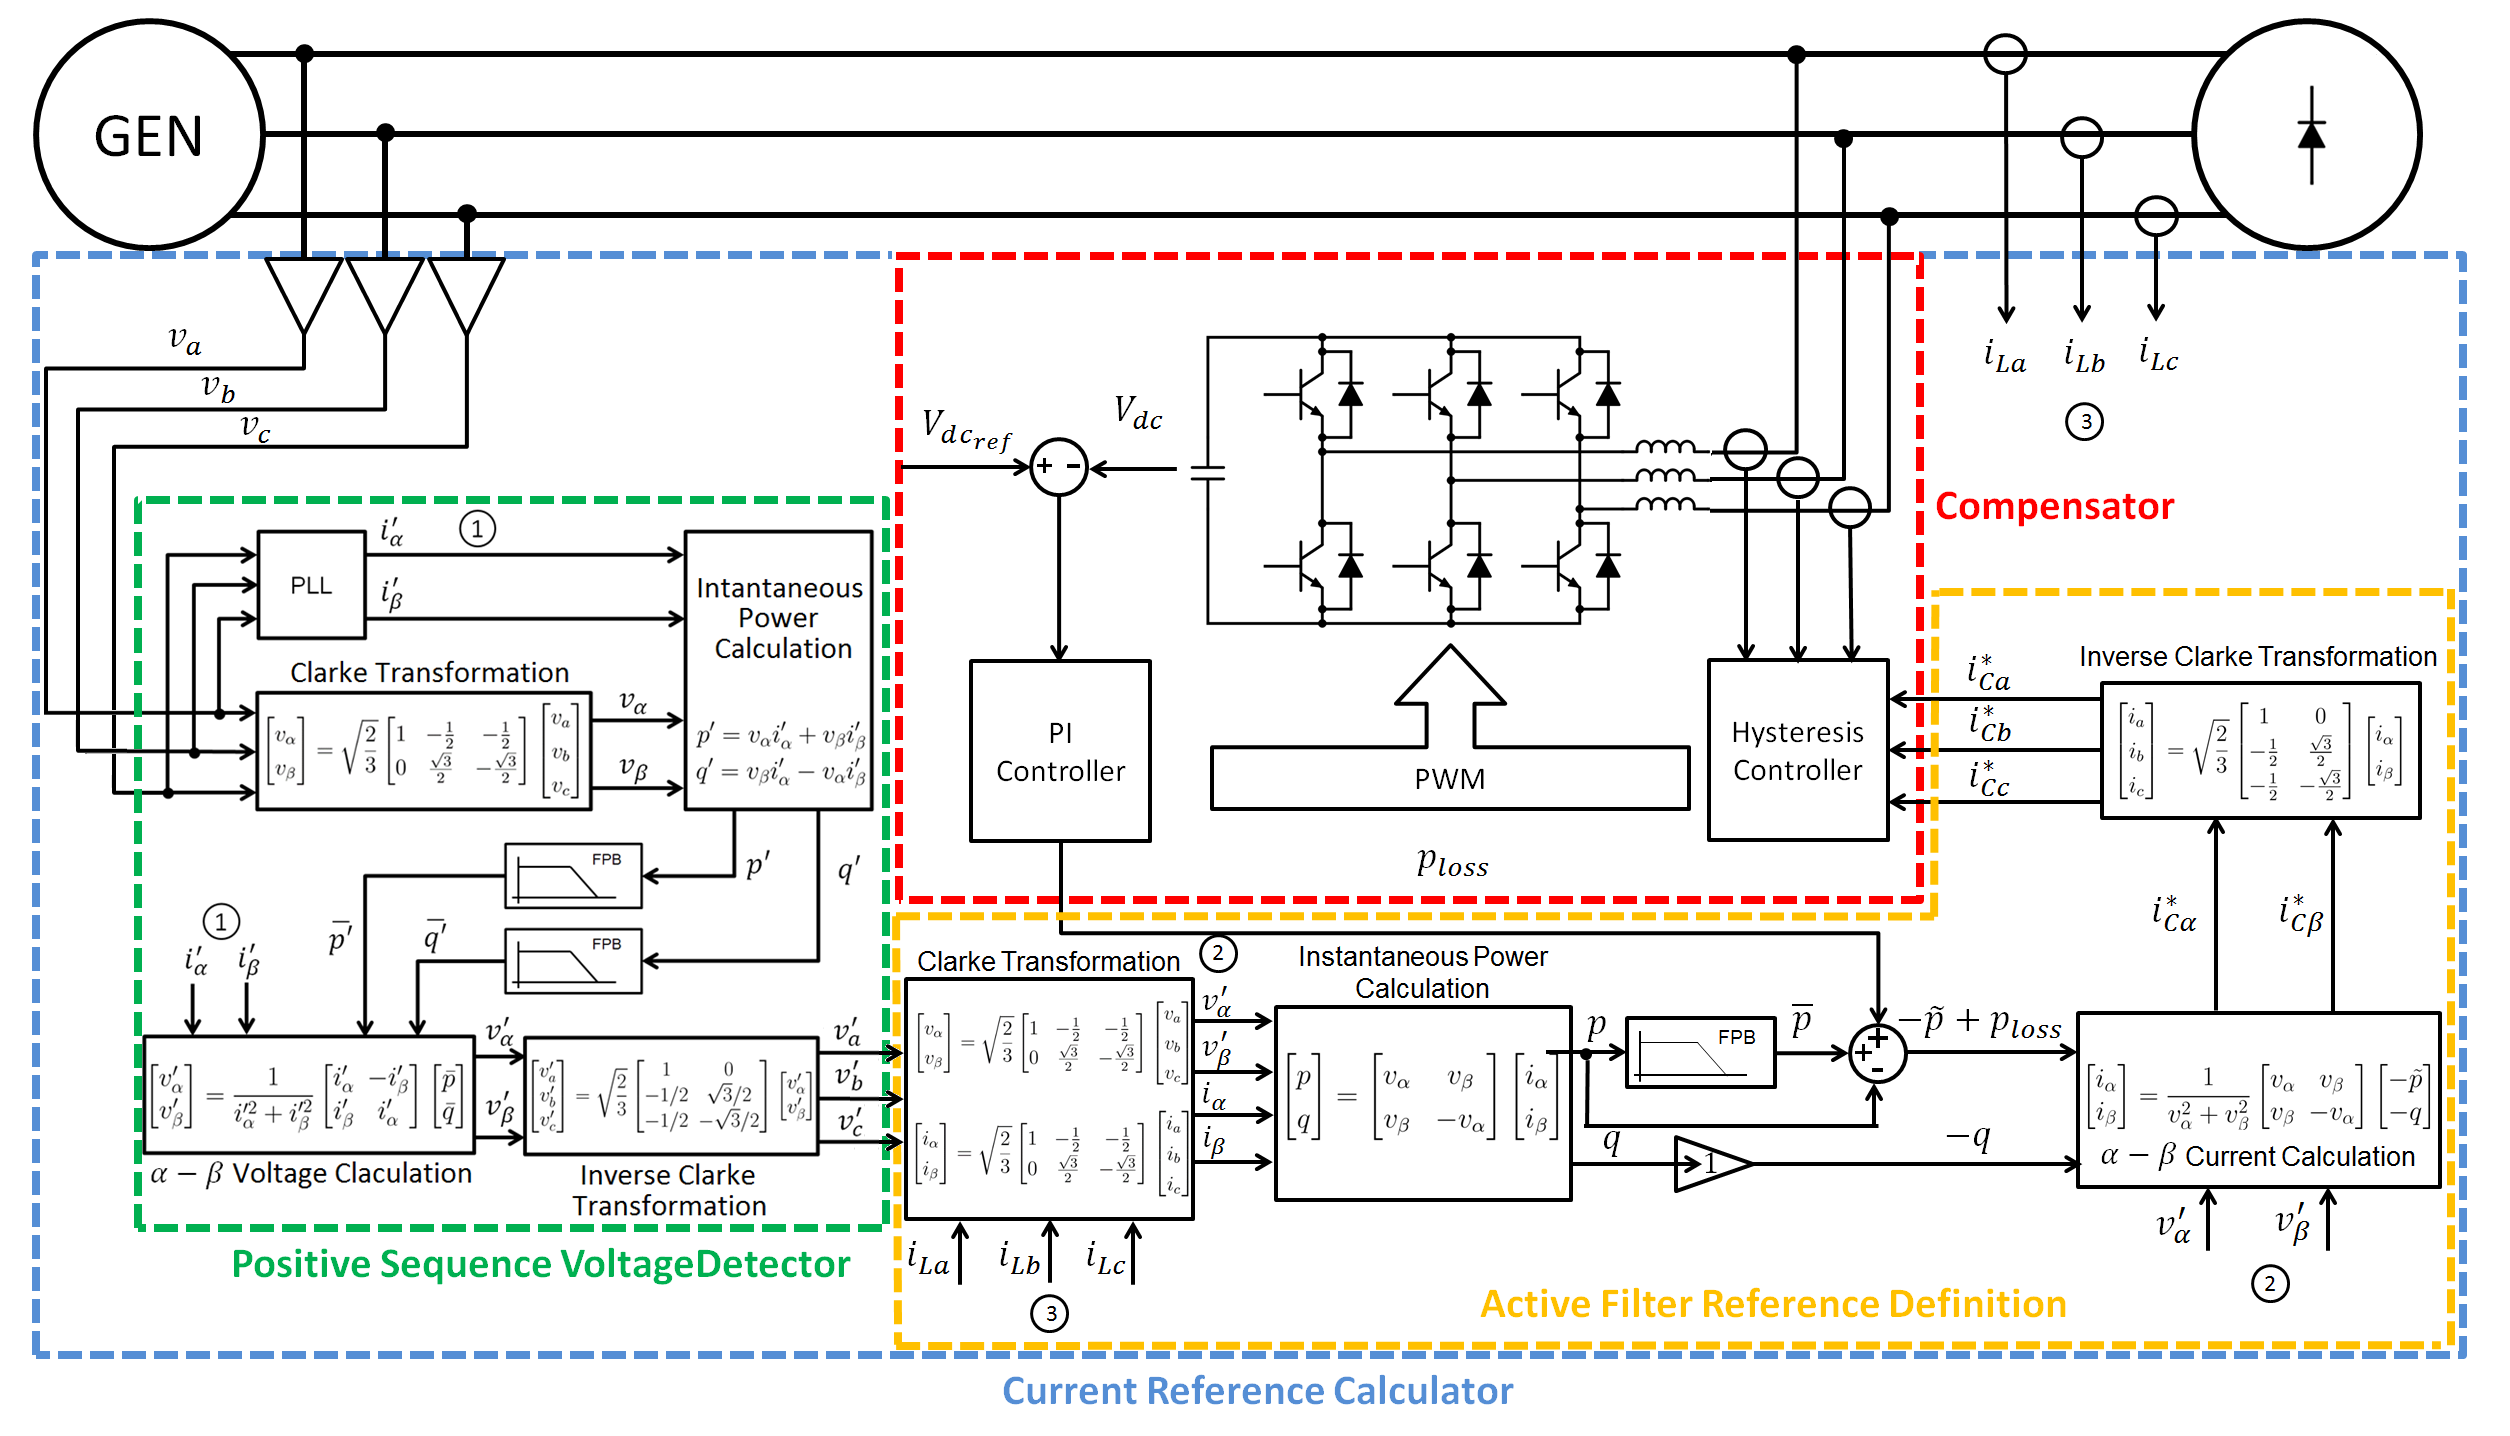
\includegraphics[width=0.83\textwidth]{Figures/filtro_blocos_1.png}
	\caption{Shunt active filter scheme}
	\label{fig:filtro_blocos_1.png}
\end{figure*}

\subsection{Electrical System Model}

The aircraft electrical system model considers the operation of the generation and distribution system with its respective non-idealities, which affect the power quality due to voltage drop. The simulation has a generator system, a power distribution system and three EHAs connected in parallel as the loads, see Fig. \ref{fig:simulacao_simulink.png}.

The generator system consists of a synchronous machine and a generator control unit (GCU). The GCU works as a field excitation controller to set the proper voltage in the PCC. The synchronous machine also has resistive and inductive reactance connected in series with the voltage source to model the resistance and the inductance presented in the generator coils.

The power distribution system is composed by the transmission lines between the generator and the PCC and between the PCC and EHAs. Probes in the PCC measure the system voltages levels to be sent as the reference input to the GCU. The power transmission lines are modeled as resistive and inductive reactance in series for each of the 3 phase lines.

The EHA controls the latero-directional and longitudinal aerodynamics surfaces. This equipment is a non-linear load, since its input has a 3-phase diode bridge. The EHAs model has a 3 phase Graetz diode bridge with a controlled current source placed in its respective DC side. The controlled current source operation recreates the apparent power consumption of a real EHA. Thereby, this guarantees the simulation of the distorted current waveforms generated by the EHA in real operation.

\begin{figure*}[!tb] %
	\centering
	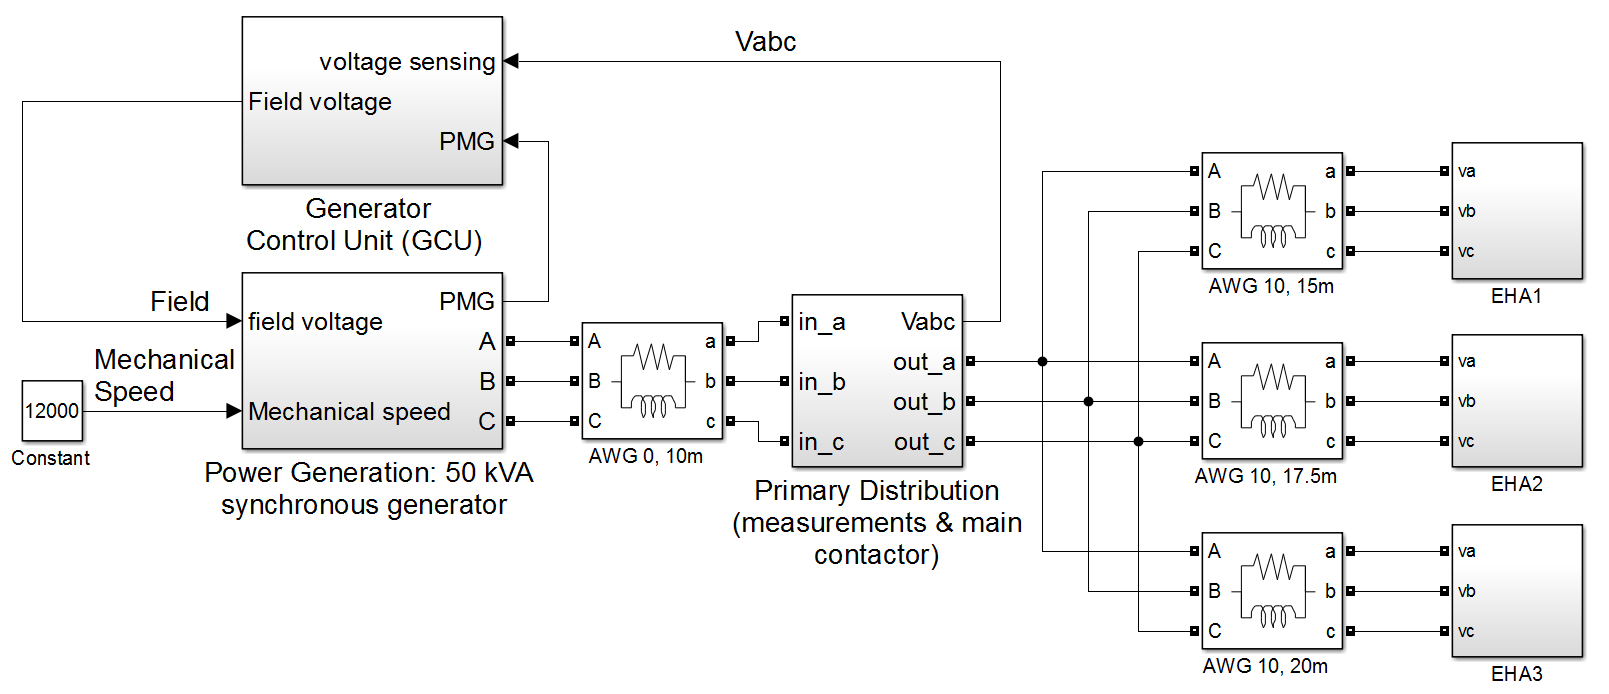
\includegraphics[width=0.6\textwidth]{Figures/simulacao_simulink.png}
	\caption{Electrical generation and distribution model}
	\label{fig:simulacao_simulink.png}
\end{figure*}

\subsection{Results}

The simulation results show the voltages and currents waveforms measured in the PCC, the voltage frequency spectrum, the amplitude constraints defined by the MIL-STD 704F, and the calculated value of the voltage THD and IHC.

The test is divided in two conditions:  the EHAs without operating and the EHAs starting their operation (maximum load). The results also show the cases where the active filters are connected and disconnected from the EHAs power input.

Fig. \ref{fig:artigo_unfilt_1.eps} and Fig. \ref{fig:artigo_unfilt_2.eps} show the system waveforms without active filters in the EHAs power inputs, when the EHAs are not in operation. Fig. \ref{fig:artigo_filt_1.eps} and Fig. \ref{fig:artigo_filt_2.eps} show the waveforms with the active filters connected to the EHAs power input for the same period. The active filters degrade the power quality during this time interval, since the THD increases and the frequency spectrum presents more harmonic content. This noise inserted in the system is due to the commutation of the VSC switching devices. Thus, even with the presence of the capacitor filter in the lines, some high frequency content injected in the grid was observed. However, the results are inside the limits defined by aeronautical standards.

Fig. \ref{fig:artigo_unfilt_3.eps} and Fig. \ref{fig:artigo_unfilt_4.eps} show the system waveforms without active filters connected to the grid, with the EHAs requiring maximum current. In the same time interval, Fig. \ref{fig:artigo_filt_3.eps} and Fig. \ref{fig:artigo_filt_4.eps} show the waveforms with the active filters connected to the EHAs power input. During this interval, it is clear the active filter enhancement in the system power quality. Considering these results, the active filter mitigates the harmonic content and set it within the limits of the MIL-STD 704F.

\begin{figure}[!h] %
	\centering
	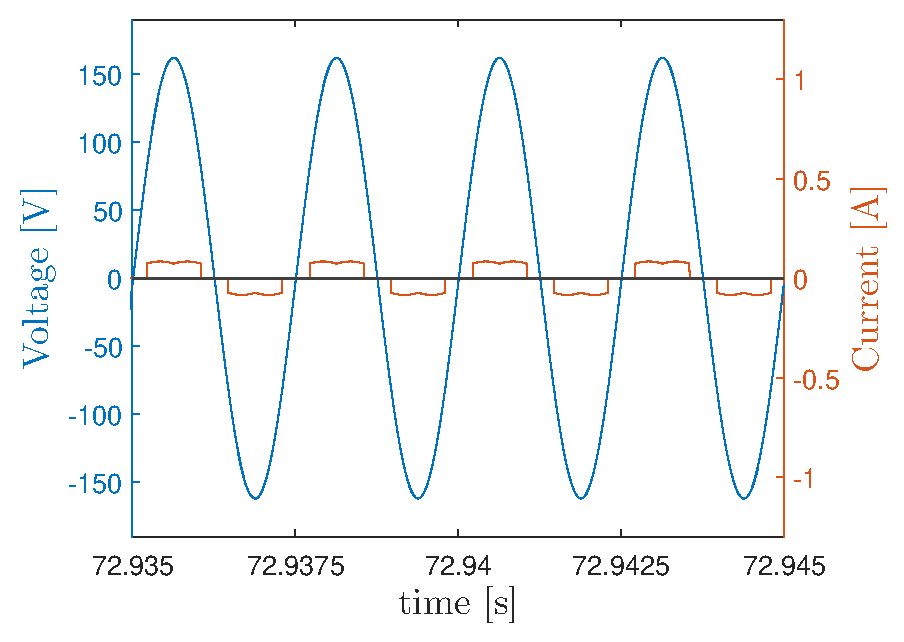
\includegraphics[width=0.27\textheight]{Figures/artigo_unfilt_1.eps}
	\caption{Voltage and current waveforms for the system without load and filter}
	\label{fig:artigo_unfilt_1.eps}
\end{figure}

\begin{figure}[!h] %
	\centering
	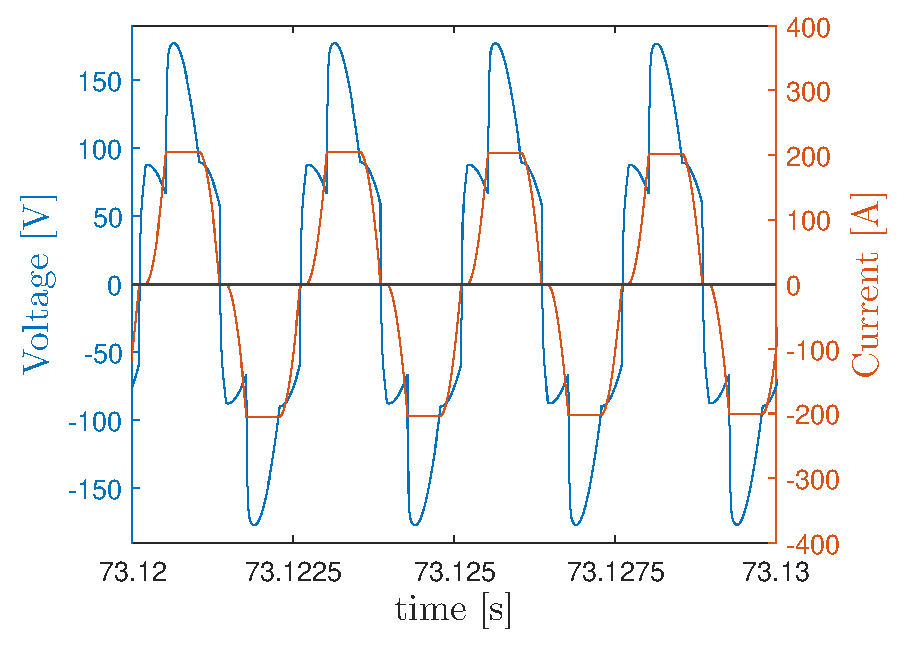
\includegraphics[width=0.27\textheight]{Figures/artigo_unfilt_2.eps}
	\caption{Voltage spectrum for the system without load and filter}
	\label{fig:artigo_unfilt_2.eps}
\end{figure}

\begin{figure}[!h] %
	\centering
	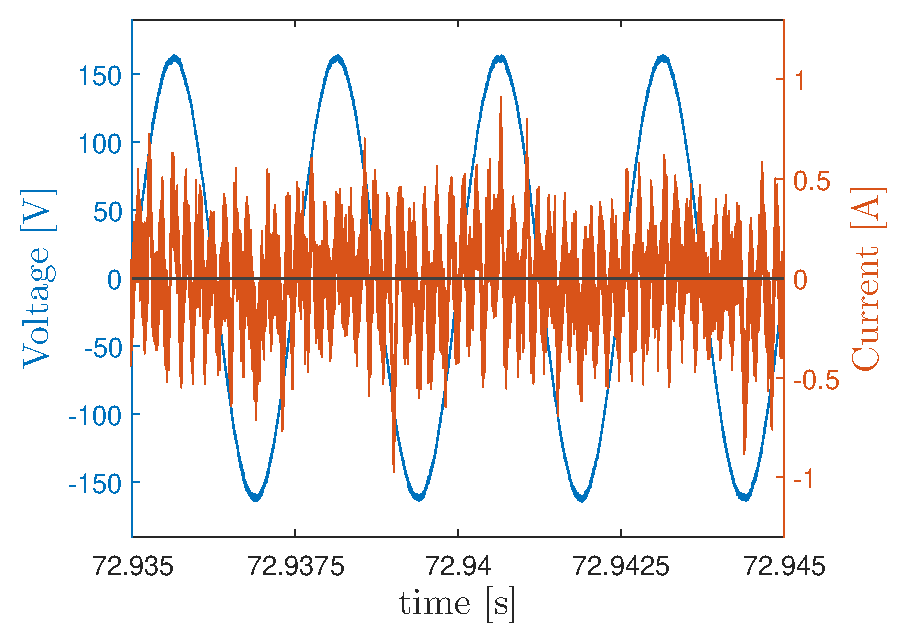
\includegraphics[width=0.27\textheight]{Figures/artigo_filt_1.eps}
	\caption{Voltage and current waveforms for the system without load and with filter}
	\label{fig:artigo_filt_1.eps}
\end{figure}

\begin{figure}[!h] %
	\centering
	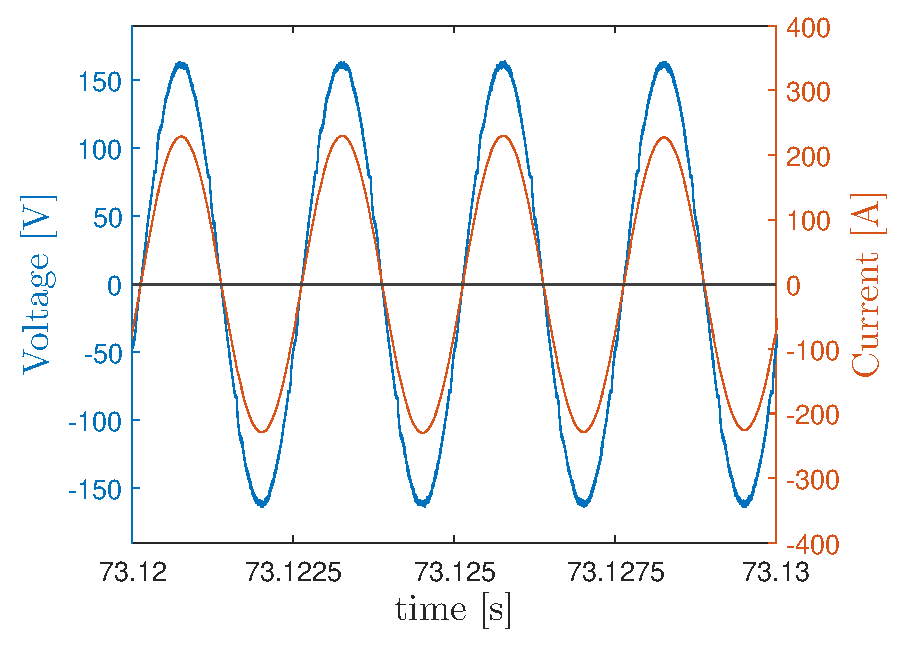
\includegraphics[width=0.27\textheight]{Figures/artigo_filt_2.eps}
	\caption{Voltage spectrum for the system without load and with filter}
	\label{fig:artigo_filt_2.eps}
\end{figure}

\begin{figure}[!h] %
	\centering
	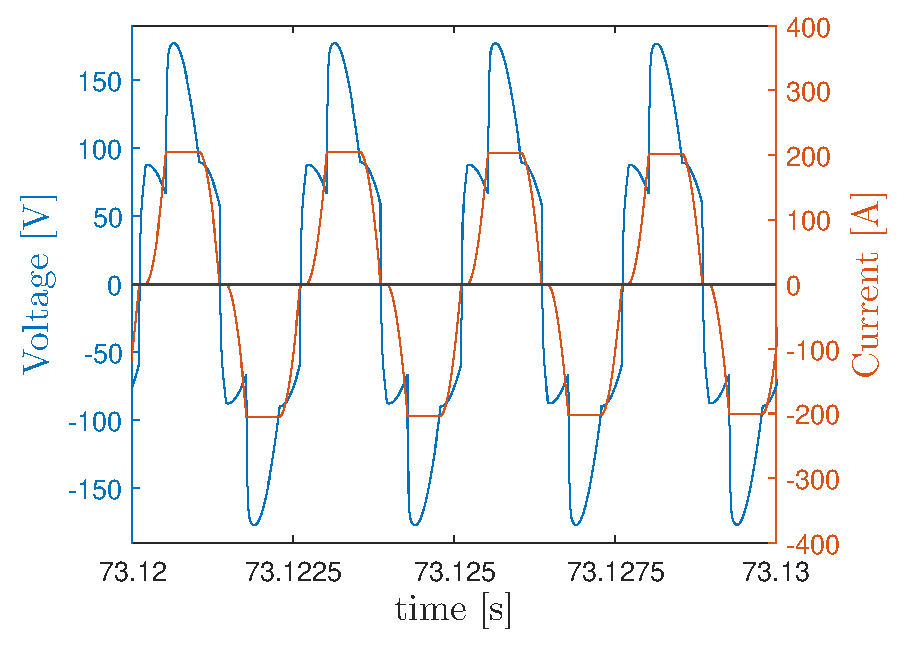
\includegraphics[width=0.27\textheight]{Figures/artigo_unfilt_3.eps}
	\caption{Voltage and current waveforms for the system with load and without filter}
	\label{fig:artigo_unfilt_3.eps}
\end{figure}

\begin{figure}[!h] %
	\centering
	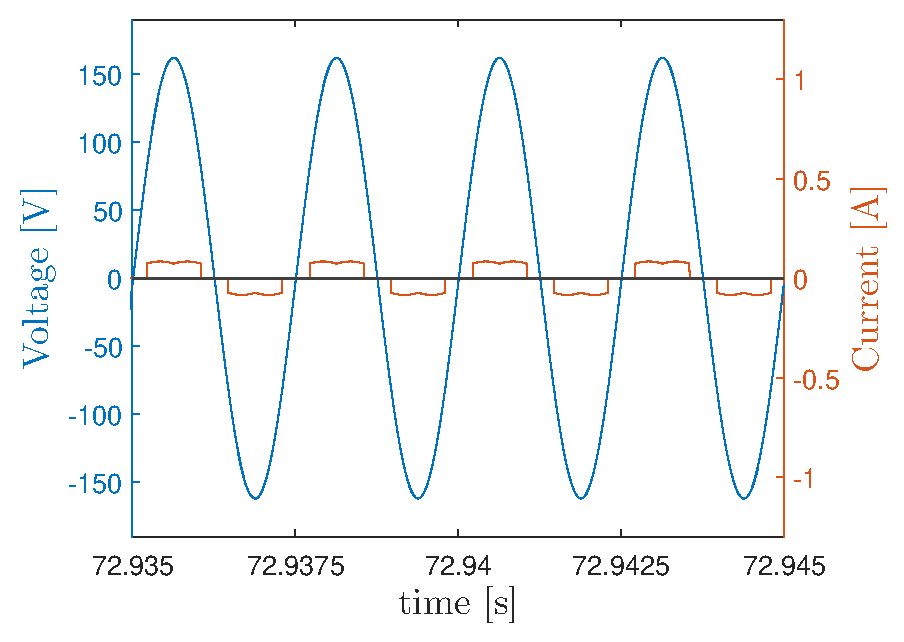
\includegraphics[width=0.27\textheight]{Figures/artigo_unfilt_4.eps}
	\caption{Voltage spectrum for the system with load and without filter}
	\label{fig:artigo_unfilt_4.eps}
\end{figure}

\begin{figure}[!h] %
	\centering
	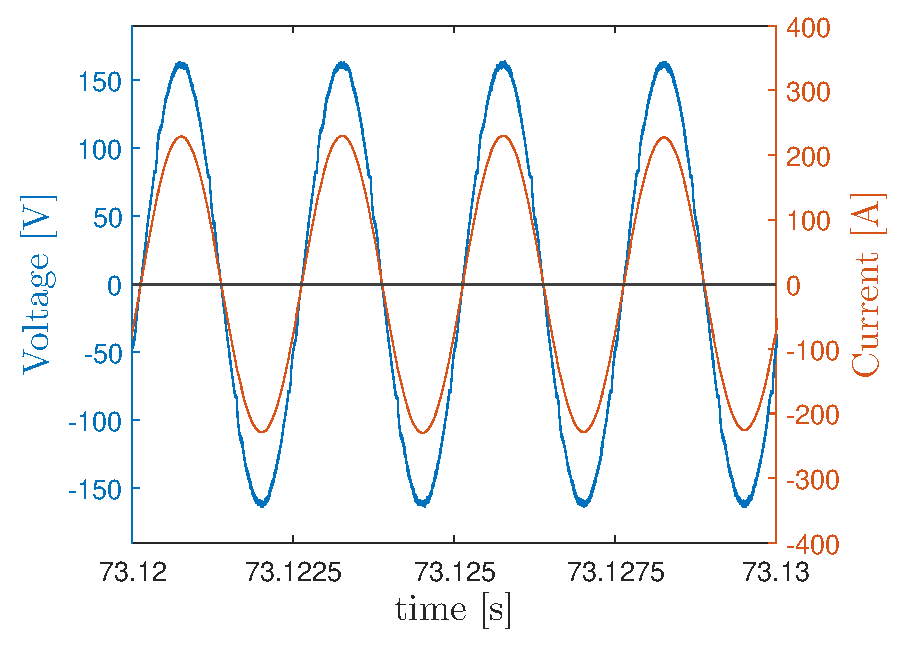
\includegraphics[width=0.27\textheight]{Figures/artigo_filt_3.eps}
	\caption{Voltage and current waveforms for the system with load and filter}
	\label{fig:artigo_filt_3.eps}
\end{figure}

\begin{figure}[!h] %
	\centering
	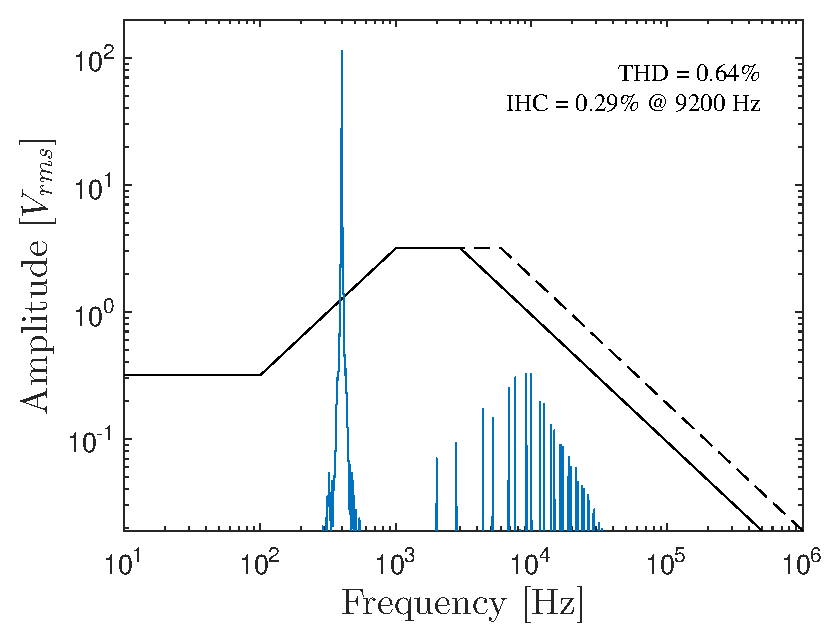
\includegraphics[width=0.27\textheight]{Figures/artigo_filt_4.eps}
	\caption{Voltage spectrum for the system with load and filter}
	\label{fig:artigo_filt_4.eps}
\end{figure}

\section{Conclusions}

\todo[inline]{sintetizar uma breve conclusão derivada da dissertação}

Com base em tudo que foi escrito, enfatize a sua contribuição sem exageros.
Trabalhos futuros, deixe-os para um outro artigo. Concentre-se no que foi realizado.

\todo[inline]{Traduzir as Figuras}

%\subsection{Subsection Heading Here}
%\blindtext

% needed in second column of first page if using \IEEEpubid
%\IEEEpubidadjcol

% An example of a floating figure using the graphicx package.
% Note that \label must occur AFTER (or within) \caption.
% For figures, \caption should occur after the \includegraphics.
% Note that IEEEtran v1.7 and later has special internal code that
% is designed to preserve the operation of \label within \caption
% even when the captionsoff option is in effect. However, because
% of issues like this, it may be the safest practice to put all your
% \label just after \caption rather than within \caption{}.
%
% Reminder: the "draftcls" or "draftclsnofoot", not "draft", class
% option should be used if it is desired that the figures are to be
% displayed while in draft mode.
%
%\begin{figure}[!t]
%\centering
%\includegraphics[width=2.5in]{myfigure}
% where an .eps filename suffix will be assumed under latex, 
% and a .pdf suffix will be assumed for pdflatex; or what has been declared
% via \DeclareGraphicsExtensions.
%\caption{Simulation Results}
%\label{fig_sim}
%\end{figure}

% Note that IEEE typically puts floats only at the top, even when this
% results in a large percentage of a column being occupied by floats.


% An example of a double column floating figure using two subfigures.
% (The subfig.sty package must be loaded for this to work.)
% The subfigure \label commands are set within each subfloat command, the
% \label for the overall figure must come after \caption.
% \hfil must be used as a separator to get equal spacing.
% The subfigure.sty package works much the same way, except \subfigure is
% used instead of \subfloat.
%
%\begin{figure*}[!t]
%\centerline{\subfloat[Case I]\includegraphics[width=2.5in]{subfigcase1}%
%\label{fig_first_case}}
%\hfil
%\subfloat[Case II]{\includegraphics[width=2.5in]{subfigcase2}%
%\label{fig_second_case}}}
%\caption{Simulation results}
%\label{fig_sim}
%\end{figure*}
%
% Note that often IEEE papers with subfigures do not employ subfigure
% captions (using the optional argument to \subfloat), but instead will
% reference/describe all of them (a), (b), etc., within the main caption.


% An example of a floating table. Note that, for IEEE style tables, the 
% \caption command should come BEFORE the table. Table text will default to
% \footnotesize as IEEE normally uses this smaller font for tables.
% The \label must come after \caption as always.
%
%\begin{table}[!t]
%% increase table row spacing, adjust to taste
%\renewcommand{\arraystretch}{1.3}
% if using array.sty, it might be a good idea to tweak the value of
% \extrarowheight as needed to properly center the text within the cells
%\caption{An Example of a Table}
%\label{table_example}
%\centering
%% Some packages, such as MDW tools, offer better commands for making tables
%% than the plain LaTeX2e tabular which is used here.
%\begin{tabular}{|c||c|}
%\hline
%One & Two\\
%\hline
%Three & Four\\
%\hline
%\end{tabular}
%\end{table}


% Note that IEEE does not put floats in the very first column - or typically
% anywhere on the first page for that matter. Also, in-text middle ("here")
% positioning is not used. Most IEEE journals use top floats exclusively.
% Note that, LaTeX2e, unlike IEEE journals, places footnotes above bottom
% floats. This can be corrected via the \fnbelowfloat command of the
% stfloats package.



%\section{Conclusion}
%\blindtext





% if have a single appendix:
%\appendix[Proof of the Zonklar Equations]
% or
%\appendix  % for no appendix heading
% do not use \section anymore after \appendix, only \section*
% is possibly needed

% use appendices with more than one appendix
% then use \section to start each appendix
% you must declare a \section before using any
% \subsection or using \label (\appendices by itself
% starts a section numbered zero.)
%


%\appendices
%\section{Proof of the First Zonklar Equation}
%Some text for the appendix.
%
%% use section* for acknowledgement
\section*{Acknowledgment}


The authors would like to thank...


% Can use something like this to put references on a page
% by themselves when using endfloat and the captionsoff option.
\ifCLASSOPTIONcaptionsoff
  \newpage
\fi



% trigger a \newpage just before the given reference
% number - used to balance the columns on the last page
% adjust value as needed - may need to be readjusted if
% the document is modified later
%\IEEEtriggeratref{8}
% The "triggered" command can be changed if desired:
%\IEEEtriggercmd{\enlargethispage{-5in}}

% references section

% can use a bibliography generated by BibTeX as a .bbl file
% BibTeX documentation can be easily obtained at:
% http://www.ctan.org/tex-archive/biblio/bibtex/contrib/doc/
% The IEEEtran BibTeX style support page is at:
% http://www.michaelshell.org/tex/ieeetran/bibtex/
%\bibliographystyle{IEEEtran}
% argument is your BibTeX string definitions and bibliography database(s)
%\bibliography{IEEEabrv,../bib/paper}
%
% <OR> manually copy in the resultant .bbl file
% set second argument of \begin to the number of references
% (used to reserve space for the reference number labels box)
\begin{thebibliography}{1}

\bibitem{IEEEhowto:kopka}
H.~Kopka and P.~W. Daly, \emph{A Guide to \LaTeX}, 3rd~ed.\hskip 1em plus
  0.5em minus 0.4em\relax Harlow, England: Addison-Wesley, 1999.

\end{thebibliography}

% biography section
% 
% If you have an EPS/PDF photo (graphicx package needed) extra braces are
% needed around the contents of the optional argument to biography to prevent
% the LaTeX parser from getting confused when it sees the complicated
% \includegraphics command within an optional argument. (You could create
% your own custom macro containing the \includegraphics command to make things
% simpler here.)
%\begin{biography}[{\includegraphics[width=1in,height=1.25in,clip,keepaspectratio]{mshell}}]{Michael Shell}
% or if you just want to reserve a space for a photo:

\begin{IEEEbiography}[{
\includegraphics[width=1in,height=1.25in,clip,keepaspectratio]{picture}}]{John Doe}
\blindtext
\end{IEEEbiography}

% You can push biographies down or up by placing
% a \vfill before or after them. The appropriate
% use of \vfill depends on what kind of text is
% on the last page and whether or not the columns
% are being equalized.

%\vfill

% Can be used to pull up biographies so that the bottom of the last one
% is flush with the other column.
%\enlargethispage{-5in}



% that's all folks
\end{document}


